\section{Graph Databases}
Un graph database é un data storage engine che combina le strutture base di un grafo con vertici e archi con un linguaggio di attraversamento (che finora abbiamo chiamato traversal) per creare un database per immagazzinare e avere rapido accesso a dati fortemente connessi. 
\begin{itemize}
    \item entities e relationships hanno equal importance
    \item meno rigido rispetto ai comuni rdbms tabellari
    \item nessun limite al numero di relazioni che puó avere un singolo nodo
    \item i nodi e gli archi possono avere piú caratteristiche che li descrivono
\end{itemize}
I database relazionali sono poco adatti a rappresentare relazioni complesse. Le relazioni in questi database sono rappresentate da chiavi esterne, che costituiscono dei puntatori a chiavi primarie in altre tabelle.
\\
Questi puntatori non sono entità che possiamo osservare o manipolare facilmente. Infatti, le chiavi esterne vengono seguite (al momento della query) da una riga a un'altra riga.
\\
I database a grafo, invece, forniscono strumenti eccellenti per navigare tra le relazioni presenti nei dati. Attribuendo alle connessioni (gli archi) un'importanza pari a quella degli elementi (i nodi), i database a grafo rappresentano tali associazioni come costrutti a pieno titolo del database, che possono essere osservati e manipolati con facilità.
\begin{figure}[th]
    \centering
    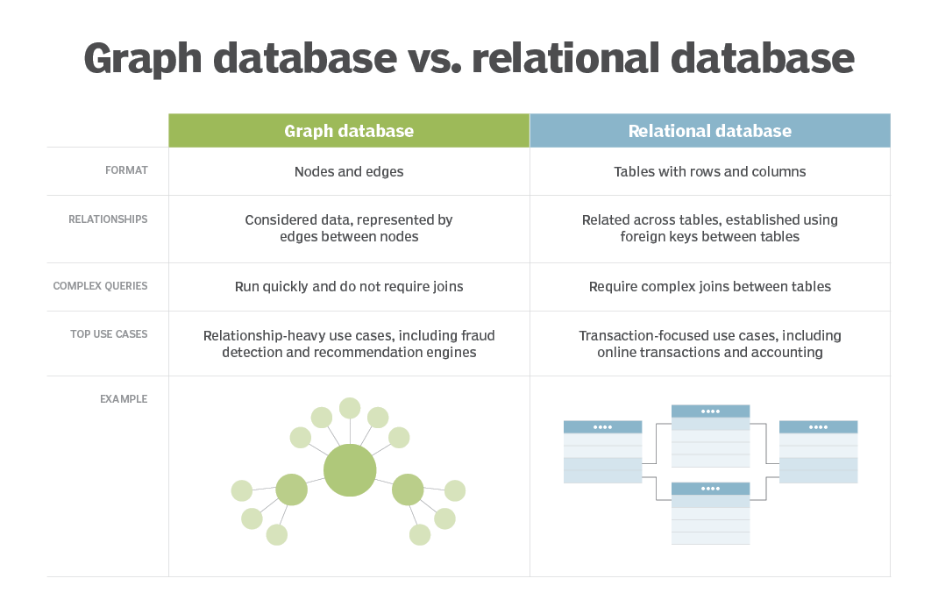
\includegraphics[scale=0.5]{GraphDatabase//img/graphvsrdbms.png}
\end{figure}
\paragraph{Advantages} Rispetto ad un RDBMS, un graph-based ha soluzioni piú efficienti in:
\begin{itemize}
    \item \textbf{query ricorsive}: per esempio, in un relational sono eseguite richiamandosi finché non arrivano al risultato desiderato; nei graph sono piú semplici da gestire con gli edges. 
    \\
    \textbf{Esempio.}  Sia data una query di questo tipo:
    \begin{verbatim}
        CREATE TABLE org_chart (
    manager_employee_id SM
    ALLINT NULL,
    employee_name
    VARCHAR(20)
    NOT NULL
    );
    \end{verbatim}
    Che genera la seguente tabella:
    \\
    \begin{figure}[th]
        \centering
        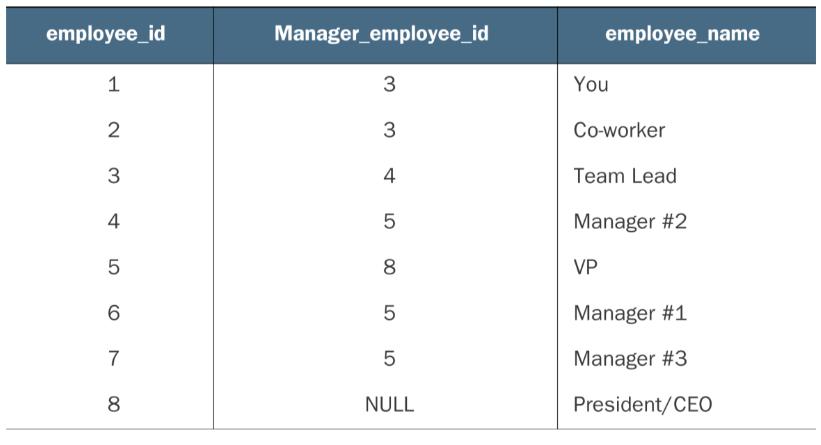
\includegraphics[scale=0.4]{GraphDatabase//img/tabellaesempio.png}
    \end{figure}
    \\
    Per costruire una gerarchia aziendale da questa tabella usando una funzione ricorsiva, in SQL:
    \begin{verbatim}
            WITH RECURSIVE org AS (
    SELECT employee_id, manager_employee_id,
    employee_name, 1 AS level
    FROM org_chart
    UNION
    SELECT e.employee_id, e.manager_employee_id,
    e.employee_name, m.level + 1 AS level
    FROM org_chart AS e
    INNER JOIN org AS m
    ON e.manager_employee_id = m.employee_id
    )
    SELECT employee_id, manager_employee_id, employee_name
    FROM org
    ORDER BY level ASC;
    \end{verbatim}
    Mentre in un graph-based la traversal query:
    \begin{verbatim}
        g.V().repeat(
        'works_for')).path().next()
    \end{verbatim}
    Con una struttura a grafo del tipo:
    \\
    \begin{figure}[th]
        \centering
        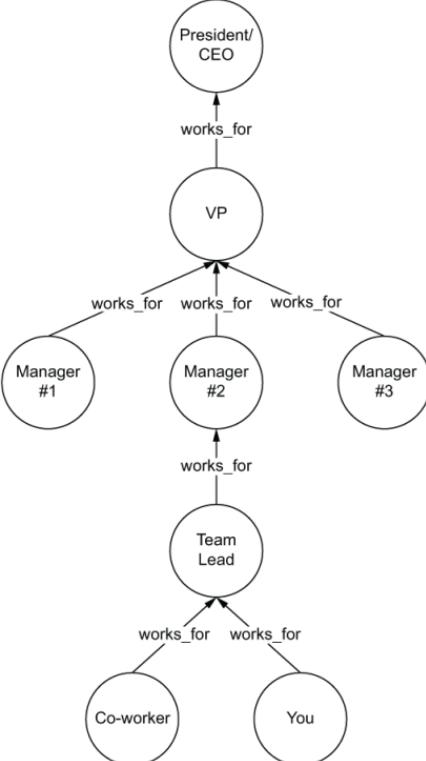
\includegraphics[scale=0.3]{GraphDatabase//img/grafoesempio.png}
    \end{figure}
    \\
    \textbf{Importante: é un esempio. Non é necessario che sia corretto ma é per mostrarne l'efficienza.}
    \item \textbf{risultati di diverso tipo}: fa riferimento a quei casi in cui vogliamo come risultato dei dati che provengono da tabelle diverse, linkate, ottenuti simultaneamente in una nuova tabella risultato (esempio: lista acquisti insieme ai product information). In un graph based i dati sono contenuti in due nodi diversi, per ottenerli basta scorrere (traversal) il grafo. 
    \item \textbf{paths}: questa é una feature esclusiva dei grafi; solo loro possono creare dei percorsi che possono essere utilizzati a nostro vantaggio per ottenere dati rapidamente.
\end{itemize}

\paragraph{Potential Issues} I contro dei graph database sono principalmente:
\begin{itemize}
    \item I database a grafo richiedono implementazioni più rigorose delle misure di \textbf{sicurezza e di accesso}. Poiché sono orientati principalmente alla mappatura delle relazioni, questa struttura può anche essere sfruttata in modi che sollevano preoccupazioni in merito alla privacy. Ad esempio, essa può offrire una visione più esplicita di un cliente o utente, e potenzialmente di tutti gli altri clienti o utenti con cui è in qualche modo collegato.
    \item Per quanto riguarda \textbf{l'integrità dei dati}, i database a grafo semplificano le modalità con cui le informazioni si relazionano tra loro. In questo processo, accorciando o condensando il percorso tra le informazioni (in confronto al dover attraversare molteplici tabelle in un database relazionale), diventa particolarmente importante garantire che tutti i dati presenti nel grafo siano accurati. Una singola relazione mal configurata può condurre direttamente a dati errati, diversamente da un database relazionale dove un dato incorretto potrebbe generare un errore durante una query annidata, rivelando così il problema. Pertanto, l'integrità dei dati assume un'importanza particolarmente elevata quando si utilizzano database a grafo.
\end{itemize}

\subsection{Tipi di Databases}
Esistono diversi tipi di graph databases:
\begin{itemize}
    \item \textbf{Property Graph Databases:} é il piú comune, salva dati come nodi e archi e dá la possibilitá di assegnare properties ad entrambi. 
    \begin{figure}[th]
        \centering
        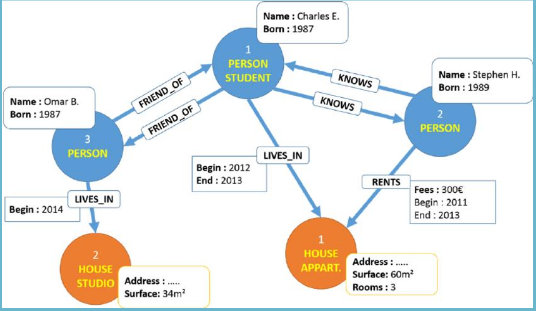
\includegraphics[width=0.5\linewidth]{GraphDatabase//img/propertygraphdb.png}
    \end{figure}
    \item \textbf{Resource Description Framework Graph Database:} usa appunto il resource description model, che rappresenta i dati come triplets formati da \textbf{nome}, \textbf{predicato} e \textbf{oggetto}.
    \begin{figure}[th]
        \centering
        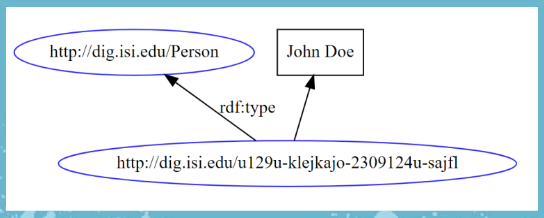
\includegraphics[width=0.5\linewidth]{GraphDatabase//img/RDF.png}
    \end{figure}
    \item \textbf{Hypergraph Database:} contiene archi e iperarchi, ovvero archi che collegano tra loro piú di due nodi, cioé crea \textbf{insiemi} di nodi.
    \begin{figure}[th]
        \centering
        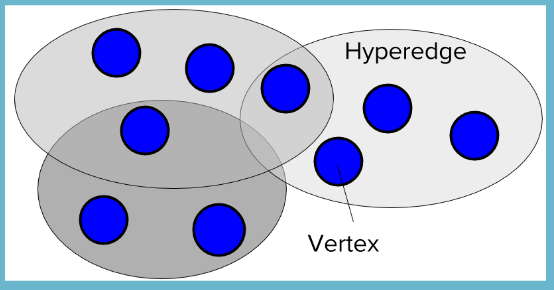
\includegraphics[width=0.5\linewidth]{GraphDatabase//img/hyperedge.png}
    \end{figure}
    \item \textbf{Spatial Graph Database:} progettato per rappresentare dati spaziali. Ad ogni nodo corrisponde una location e gli edges rappresentano relazioni tra due punti. Supporta spatial indexing e spatial querying.
    \\
    \begin{figure}[th]
        \centering
        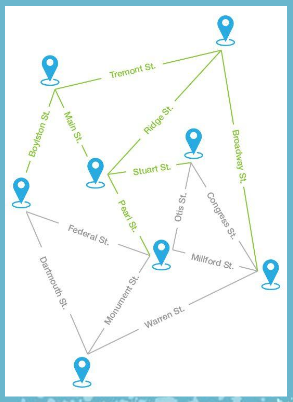
\includegraphics[width=0.25\linewidth]{GraphDatabase//img/positionaldb.png}
    \end{figure}
    \item \textbf{Temporal Graph Databases:} progettato per rappresentare dati temporali, come time series o event logs. Ad ogni nodo corrisponde una entity e gli edges rappresentano relazioni tra due punti in uno specifico istante.
    \\
    \begin{figure}[th]
        \centering
        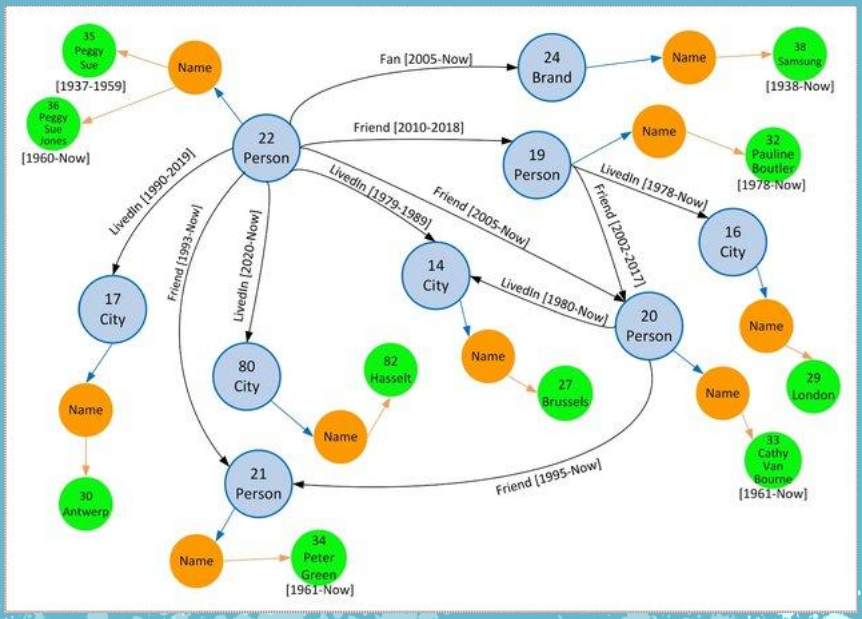
\includegraphics[width=0.45\linewidth]{GraphDatabase//img/temporaldb.png}
    \end{figure}
    \item \textbf{Property-Graph Triplestore Hybrid:} combina property e RDF.
    \\
    \begin{figure}[th]
        \centering
        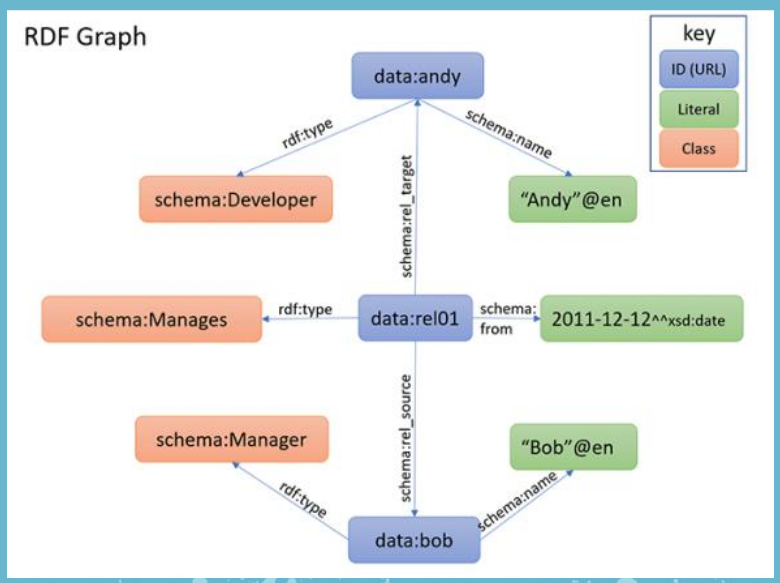
\includegraphics[width=0.35\linewidth]{GraphDatabase//img/rdfmixdb.png}
    \end{figure}
\end{itemize}

\newpage

\subsection{Graph Landscape}
Negli ultimi anni sono emersi numerosi progetti e prodotti per la gestione, l'elaborazione e l'analisi dei grafi. L'elevato numero di tecnologie rende difficile tenere traccia di tutti questi strumenti e comprendere in che modo si differenziano.
\\
Possiamo suddividere lo spazio delle tecnologie grafiche in due categorie principali:

\begin{enumerate}
    \item Le tecnologie utilizzate principalmente per la persistenza transazionale dei grafi in tempo reale, generalmente accessibili direttamente durante l’esecuzione. Queste sono chiamate \emph{graph databases}, e sono l’equivalente dei database OLTP.
    \item Le tecnologie utilizzate principalmente per l'analisi offline dei grafi, eseguita tipicamente come una serie di passaggi batch. Queste sono chiamate \emph{graph compute engines}, e sono analoghe ai processi di data mining e OLAP.
\end{enumerate}
\subsubsection*{Il sistema di archiviazione sottostante}

Alcuni database a grafo utilizzano un sistema di archiviazione nativo per i grafi, ottimizzato e progettato specificamente per memorizzare e gestire dati strutturati come grafi. \\
Tuttavia, non tutte le tecnologie di database a grafo adottano una memorizzazione nativa. Alcune serializzano i dati del grafo all'interno di un database relazionale, orientato agli oggetti o in un altro tipo di archivio dati generico.
\\
\begin{figure}[th]
    \centering
    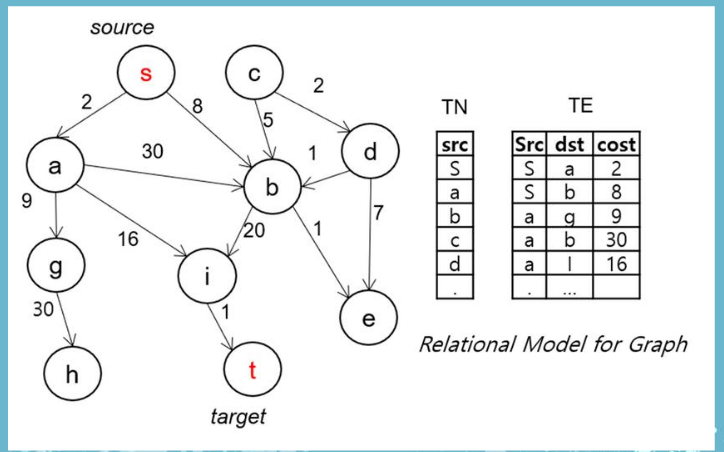
\includegraphics[width=0.5\linewidth]{GraphDatabase//img/immagine1.png}
\end{figure}

\subsubsection*{Aderenza senza indice nei database a grafo}

Un database a grafo utilizza il concetto di \emph{index-free adjacency}, ovvero l'adiacenza priva di indice, il che significa che i nodi connessi si “puntano” fisicamente l’un l’altro all'interno del database.
\\
Ogni nodo fa riferimento diretto ai suoi nodi adiacenti, mantenendo una sorta di mini-indice locale verso i nodi vicini. Questo approccio rende le operazioni di attraversamento estremamente economiche in termini di prestazioni.
\\
Adottiamo una visione leggermente più ampia: qualsiasi database che, dal punto di vista dell'utente, si comporta come un database a grafo — cioè espone un modello di dati a grafo attraverso operazioni CRUD — può essere considerato un database a grafo.
\\
Riconosciamo tuttavia i significativi vantaggi in termini di prestazioni offerti dall’\emph{index-free adjacency} e, per questo motivo, utilizziamo il termine \emph{native graph processing} per descrivere quei database a grafo che sfruttano tale adiacenza priva di indice.

\subsubsection*{Perché scegliere Graph-Based?}
\begin{itemize}
    \item \textbf{Prestazioni}: i database a grafo offrono prestazioni superiori per le query su dati connessi, superando i database relazionali e NoSQL, specialmente con l'aumentare della quantità di dati. A differenza dei database relazionali, dove le query ricche di join rallentano con la crescita del dataset, le query nei grafi restano efficienti e localizzate.
    \item \textbf{Flessibilità}: la natura priva di schema dei grafi consente una modellazione dei dati adattiva, permettendo agli sviluppatori di evolvere dinamicamente la struttura senza necessità di complesse migrazioni o definizioni di schema anticipate.
    \item I database a grafo si allineano allo sviluppo software agile, supportando una crescita iterativa e modifiche fluide. (agility e evolving)
    \item La loro natura additiva consente di aggiungere relazioni, nodi e etichette senza compromettere le query esistenti.
    \item A differenza dei database relazionali, la governance viene applicata in modo programmatico attraverso approcci basati su test, garantendo affidabilità anche in applicazioni in continua evoluzione.
\end{itemize}

